\documentclass{VUMIFPSkursinis}
\usepackage{algorithmicx}
\usepackage{algorithm}
\usepackage{algpseudocode}
\usepackage{amsfonts}
\usepackage{amsmath}
\usepackage{bm}
\usepackage{caption}
\usepackage{color}
\usepackage{float}
\usepackage{graphicx}
\usepackage{listings}
\usepackage{subfig}
\usepackage{array}
\usepackage{wrapfig}
\usepackage{tabu}

% Titulinio aprašas
\university{Vilniaus universitetas}
\faculty{Matematikos ir informatikos fakultetas}
\department{Programų sistemų katedra}
\papertype{Kursinis darbas}
\title{Detalus vaizdų panašumas naudojant trejetų tinklus}
\titleineng{Fine-grained images similarity using triplet-network}
\status{4 kurso 6 grupės studentas}
\author{Andrius Butkevičius}
% \secondauthor{Vardonis Pavardonis} % Pridėti antrą autorių
\supervisor{dr. Vytautas Valaitis}
\date{Vilnius – \the\year }

% Nustatymai
% \setmainfont{Palemonas} % Pakeisti teksto šriftą į Palemonas (turi būti įdiegtas sistemoje)
\bibliography{bibliografija}

\begin{document}

\maketitle
\thispagestyle{empty} 

\tableofcontents


\sectionnonum{Įvadas}

\thispagestyle{empty} 
Vaizdų panašumo įvertinimas ir lyginimas tampa vis plačiau naudojamas ir susilaukia vis didesnio dėmesio informacinių technologijų srityje.Visgi plėtojant šią technologiją ir siekiant išgauti kuo korektiškesnius rezultatus yra susiduriama su problemomis, pavyzdžiui.: kaip kompiuteriui efektyviau atskirti vizualius skirtumus ir vaizdų panašumus žinant, kad kompiuterinėms mašinoms, tai nėra taip lenva, kaip palyginus žmogui, kuris gali akimirskniu sugebėti atpažinti aplink jį esamus objektus. Vaizdų identifikavimas ir jų lyginimas plačiai naudojama vaizdų klasifikavime, objektų atpažinime, pvz.: vaizdinės tapatybės nustatymui, veido atpažinimui, esamos vietovės aptikimui pasitelkient beipiločio orlaivio užfiksuotas reljefo nuotraukų, nuotraukų radimui pasitelkiant paieškos sistemas. Norint sugebėti tai atpažinti ir klasifikuoti, yra pasitelkiami įvairūs tinklų modeliai ir jie treniruojami, tokie kaip Siamese arba trejetų tinklai. Šie tinklai susideda iš dviejų ar trijų vienodų ir lygiagrečių konvoliucinių neurono tinkle esančių atšakų, kurios tarpusavyje dalinasi svoriais, kurių dėka galima gauti aukšto lygio nuotraukų bruožų atvaizdavimą taip leidžiant panašioms nuotraukoms būti kuo arčiau sujungtoms viena su kita funkcijos erdvėje. Tuo metu nepanašiems vaizdams – būnant kuo toliau nuo teisingų nuotraukų. Rinkoje yra siūlomi įvairūs konvoliucinių neuronų tinklų modeliai, pvz.: Alexnet, VGGNet, GoogLetNet, ResNet. Verta paminėti, kad visi šie modeliai turėjo efektyvius atpažinimo rezultatus ILSVRC. Taigi vis dažniau yra pasitelkiama prieš tai minėti trejetų tinklai, kurie optimizuoja bruožų atstumus erdvėje. Visgi sudėtingiausia problema išlieka dėl semantinio tarpo problemos, kuri atsiranda tarp žemos rezoliucijos nuotraukos pikselių užfiksuotų kompiuterinių sistemų ir aukšo lygio semantinių koncpetų, kurias suvokia žmonės. Dėl to reikia rasti geresnių būdų, kaip sugebėti pateikti nuotrauką kompiuteriui ir gauti gilesnias jos semantinius bruožus. Todėl šio darbo tikslas yra ištirti esamus rinkoje modelių veikimo principus, jų niuansus bei palyginimą vieną su kitu. Išanalizuoti, kada, kokiomis sąlygomis jie veikia geriausiai. Taigi bus pasirinkta viena iš esamų vaizdų duomenų rinkinių ir bus treniruojamas trejetų tinklas, analizuojamos rezultatai, problemos.

\pagebreak
\sectionnonum{Tikslas}
Šio darbo tikslas yra:
\begin{itemize}
\item{Išsiaiškinti pasirinkto trejetų tinklo modelio rezultatus, identifikuojant žmonių siluentus viešose erdvėse.}
\item{Gautus vaizdų palyginimo rezultaus paanalizuoti detaliau, išskirti jų metrikas.}
\item{Palyginti architektūrą su kitais neuronų tinklų modeliais.}
\end{itemize}
 
\sectionnonum{Uždaviniai}
\thispagestyle{empty}
\begin{enumerate}
\item{Ištreniruoti trejetų tinklų modelį atpažįstant žmonių siluetus, nufotografuotus viešoje vietoje.}
\item{ Išskirti metrikas pagal kurias galėtų analizuoti gautus rezultatus, panaudojant trejetų tinklų modelį.}
\item{Išskirti pasirinkto tyrimo rezultatų trūkumus ir išsiaiškinti galimas sritis ateities darbams.}
\item{Palyginti kitų neuronų tinklų modelių architektūras.}
\end{enumerate}

\pagebreak
\section{Trejetų ir Siamese tinklų tyrimų literatūros analizė}

\subsection{Gilieji konvoliuciniai neuronų tinklai}
Giliajame mokymese, šis tinklas yra klasė iš giliųjų neuronų tinklų, kuri dažniausiai naudojama pritaikant vaizdų atpažinimą. Tai yra algoritmas, kuris įvestyje pasiima vaidą (nuotrauką ar paveiksliuką), priskiria jam svorius ir jos bruožų tendencijas įvairiose nuotraukos dalyse ir sugeba pagal tai atskirti panašumus lyginant su kitomis nuotraukomis.

\subsection{Trejetų tinklai}
Trejetų tinklų modelis būvo pasiulytas 2014m., moksliniko Chang Wang\cite{Learning_fine_grained_image}. Modelio veikimo principas susideda iš trijų identiškų konvoliucinių neuroninių tinklų šakų, kurie tapusavyje dalijasi gautais svoriais. Kai trejetų tinklas įvestyje gauna tris pavyzdžius, išvestyje yra grąžinama dvejos tarpinės reikšmės, kurios nurodo atstumus lyginimus su pagrdine įvestimi ir kitomis dvejomis įvestimis, kurių rezultatas yra vektoriai.
\begin{figure}[H]
\centering
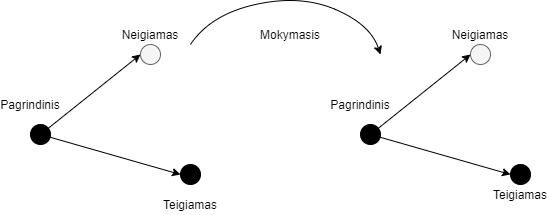
\includegraphics[scale=0.5]{img/Triplet_network}
\caption{Trejeto tinklo mokymosi procesas \cite{Improved_triplet_network}} % Antraštė įterpiama po paveikslėlio
\label{img:mlp}
\end{figure}
\pagebreak

\subsubsection{Architektūra}
Trejetų tinklų modelis įvedimo dalyje reikalauja trijų įvesčių tuo pačiu metu. Kiekvienas jų turi savo pavadinimą ir reikšmę tinkle, pagrindinis $x^a$, pozityvus $x^p$, negiamas $x^n$. Įvesties poros $x^a$ ir $x^p$ yra tos pačios kategorijos arba panašūs semantiškai įvestys. Tuo metu $x^a$ ir $x^n$ yra skirtingos kategorijos arba nepanašūs visai. Pasitelkiant funkcijas yra apskaičiuojama jų semantiniai panašumai atsumo erdvėje (nes jie yra pateikiami kaip vektoriai). Ši funkcija yra vadinama nuostolių funkcija, jos funkcija aprašyta žemiau. Kur parametras $\alpha$ rodo tarpą tarp $x^a$ ir $x^p$ bei $x^a$ ir $x^n$. $N$ reiškia skaičių nusakantį kiek trejetų įvesčių yra pateikiama. Tikslas yra pasiekti, kad $x^a$ ir $x^p$ būtų mažiau nei $x^a$ ir $x^n$ \cite{Face_recognition}.

\[loss = \sum_{x=1}^{N} max(d(x^a, x^p) - d(x^a, x^n) + \alpha, 0)\]
Kur $d$ yra atstumo metrika, taip kad $d(x^a, x^p) < d(x^a, x^n)$, o $N$ yra skaičius trejetų.

\subparagraph{Alternatyvios nuostolių funkcijos}
Artima šiai funkcijai yra ši lygtis. Ji naudoja kvadratinį Euklido \cite{Aerial_image_similarity} atstumą kaip atstumo metriką ir $\alpha > 0$, nurodanti ribą tarp dviejų vaizdų ir absoliučios sumos reikšmės.
\[loss = \sum_{x=1}^{N} [||x^a - x^p|| - ||x^a - x^n|| + \alpha]\]

\begin{figure}[H]
\centering
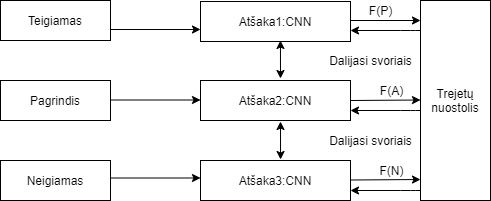
\includegraphics[scale=0.8]{img/Triplet_network_branchCNN}
\caption{Trejeto tinklų veikimo principas kartu su neuroninių tinklų lygiagrečiomis atšakomis} % Antraštė įterpiama po paveikslėlio
\label{img:mlp}
\end{figure}

Šis neuroninių tinklų architektūrinis sprendimas padeda apmokyti duomenų klasifikavimą išskaidant duomenis pagal panašumus ir skirtumus. Jų metu keli lygiagretūs gileiji neuroniai tinklai yra apmokami bei tuo pačiu metu jie dalijasi svoriais vieni su kitu treniruojant tinklą. Trejetų tinkle tikslas yra sukurti trejetus, kurie susideda iš pagrindinio $p^a$, teigiamio $x^p$, neigiamio $p^n$ − įvesties elementų. Pagrindinis elementas, tai kažkokia įvestis (nuotrauka, paveiksliukas, muzikos įrašas ir t.t), kuriai mes bandome rasti atitikimą iš kitos įvesties. Teigiama įvestis – panašus elementas atitinkamai pagrindiniai nuotraukai. Tuo tarpu neigiamas elementas skaitosi tas, kuris neturi panašumų su pagrindine nuotrauka. Neuroninai tinklai apskaičiuoja  $\pi : f(\pi) \in$
Šie trys elementai yra įvedami nepriklausomai vienas nuo kito į  tris identiškus giliuosius neuroninius tinklus, kurie dalijasi vienoda architektūra ir parametrais. Jų metu yra apskaičiuojami atstumai tarp šių elementų. Šiam apskaičiavimui yra naudojama praradimo funkcija.
\linebreak
Įmanomi rezultatai trjetų tinkle:
\begin{itemize}
\item{Lengvas trejatas: trejetai, kurie turi nuostolį, reikšme 0, nes $d(x^a, x^p) + \alpha < d(x^a, x^p)$}
\item{Sudėtingas trejetas: trejetai, kurių neigiamumas yra arčiau pagrindinio negu teigiamų, $d(x^a, x^p) < d(x^a, x^p)$}
\item{Pusiau sudėtingas trejetas: trejetai, kurių neigiamumas nėra arčiau teigiamumo, tačiau vis tiek turi teigiamą nuostolį: $d(x^a, x^n) < d(x^a, x^p) +\alpha$}
\end{itemize}

\subsection{Siamese tinklas}
Pirma kartą publikuotas 1990 metais, autorių Bromely ir Yann LeCun, siekiant išspręsti parašo verifikavimo problema kaip vaizdo atitikimo probelmą\cite{Siamese_signature_verifiction}.
\subsubsection{Architektūra}
Tinklo modelis – neuronų tinklas turintys kelis ar daugiau identiškus neuroninių tinkle atšakas su vienodais parameterais\cite{Siamese_Network}. Šis modelis naudoja vienodus svorius vykdant tuo pačiu metu ir panaudojant du skirtingus įvesties vektorius apskaičiuojant palyginamus išvesties vektorius. Šie vienodi tinklai su skiringais įvesties duomenimis yra sujungti pagal energijos funkciją $E$. Ši matematinė funkcija apdoroja kai kurias metrikas tarp labiausiai išryškintų bruožų vaizdavimų kiekvienoje pusėje.
Parametrai tarp šių vienodų tinkle yra apriboti, kad būtų vienodi. Svorių apjungimas užtikrina, kad du labai panašūs vaizdai nebūtų tarp jų atitinkamų tinkle išvesti labai skirtinguose erdvės lokacijose. Taip pat, reikia paminėti, kad tinklas yra simetriškas, nesvarbu kuriam iš vienodų tinklų įvesime vaizdą, visada gausime tokias pačias metrikas.
Standartinė išlaidų funkcija skirta mokymosi pavyzdžiui (x1,x2) yra pasiūlyta Hadselio. L(W,(Y, x1, x2)) = 1 2 (1 − Y )(D(W, x1, x2))2+ 1 2 Y max{0, m − D(W, x1, x2)} 2 (4) where D(W, x1, x2) = ||f(W, x1) − f(W, x2)||2 . Y = 1 if (x1, x2) yra panašios poros, ir Y = 1 kitu atveju. m yra riba nurodanti norimą slenkstį atstumui tarp x1 ir x2 jeigu jie nėra panašūs. Dėl laisvo suregualiavimo, dažniausiai taip yra sunkiau ištreniruoti trejetų tinklus negu Siamese tinkle.

\begin{figure}[H]
\centering
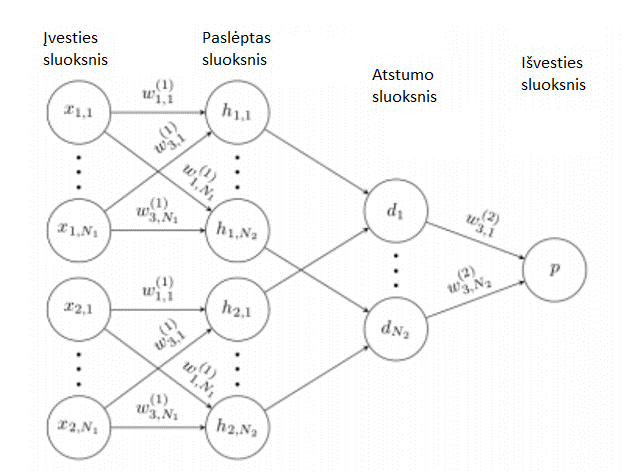
\includegraphics[scale=1.0]{img/Siamese}
\caption{Siamese tiklų modelis} % Antraštė įterpiama po paveikslėlio
\label{img:mlp}
\end{figure}

\subsection{Nefiksuoto dydžio vaizdai konvoliuciniuose tinkluose}
Gilieji konvoliuciniai tinklai reikalauja fiksuoto dydžio įvesties vaizdų. Tačiau realiame gyvenime nuotraukų ar paveiksliukų dydžiai nėra fiksuoti ir varijuoja plačiai.
\linebreak
Jeigu yra bandoma primiktynai pakeisti į reikiama dydį, nuotrauką karpant ar deformuojant, informacija, patalpinta nuotraukose bus prarasta. To pasekoje tikslumas nuotraukų klasifikacijos ar objektų identifikavime bus sumažintas ir nepataisomai sugadintas. Nors neuroniniuose tinkluose, konvoliuciniai sluoksniai nereikaljau fiksuoto dydžio įvesties ir geba generuoti specifinius bruožus vaizdo iš bet kokio dydžio nuotraukų. Visgi, pilnai sujungti sluoksniai privalo turėti fiksuoto dydžio įvestį dėl jų pačių apibrėžimo. Dėl to apribojimas fiksuoto dydžio nuotraukų ateina tik iš pilnai sujungtų sluoksnių reikiamos ypatybės.
Viena iš šios problemos sprendimo būdų yra naudoti erdvinės piramidės talpinimą\cite{Spatial_pyramid_pooling}.
\linebreak

The spatial pyramid pooling layer extracts the image features from the feature map through the 4 × 4, 2 × 2, and 1 × 1 square grid. Then, the SPP layer produces 21 = 16 + 4 + 1 different spatial bins and obtain a fixed size output by pooling each block. After the spatial pyramid pooling, any feature map can generate 5376-dimensional feature vector, where 5376 = 21 × 256. The SPP layer pools the features and generates fixed length outputs, which are then fed into the fully-connected layers. Therefore, the convolution neural network with spatial
\pagebreak

\section{Įvertinimo funkcija}
Kelios įvertinimų metrikos yra naudojamos: panašumo tikslumas bei \emph{score-at-top-K}, kai $K = 30$. Panašumo tikslumas yra išreiškiamas procentaliai pagal tai, kiek trejetų buvo korektiškai sureitinguota. Sakykime, kad turime trejetą, su šiais įvesties parametrais $tt = (x^a, x^p, x^n)$, kur $x^p$ turėtų būti arčiau(panašesnis)šalia $x^a$. Laikant, kad $x^a$ yra įvesties užklausa žiūrime į rezultatus kitų įvesties duomenų. Jeigu $x^p$ yra reitinguojamas aukščiau nei $x^n$, tai tada teigiame, kad atitinkamas trejetas yra sureitinguotas teisingai. Kita mums reikalinga metrika, kuri buvo užsiminta anksčiau \emph{score-at-top-K}. Jis nusako skaičių teisingai sureitinguotų trejetų bei atimant iš šio skaičiaus, kuris nusako neteisingai sureitinguotus trejetus iš pogrupio trejetų, kurių reitingas yra didesnis, nei kintamasis $K$. Pogrupis yra pasirenkamas tokia tvarka: kiekvienam užklausos paveikslėliui iš duomenų aibės, ištraukia 1000 naujų paveikslėlių iš tos pačios teksto užklausos ir yra bandoma taip reitinguoti juos, pasitelkiant išmoktas metrikas. Trejeto reitingas yra aukštesnis negu $K$, jeigu jo $x^p$ arba $x^n$ yra tarp geriasiai reitinguojamų $K$ kaimynų iš užklausos su paveikslėlių $x^a$.
\pagebreak

\subsection{Treniruojami duomenys}
Kadangi darbo tema susijusi su detalių vaizdų panašumu, kuris negali būti charakterizuotas pagal paveikslėlių žymes, buvo panaudota trejetų duomenų rinkinys įvertinant vaizdo panašumo modeliams.
Buvo paimta 1000 populiariausių teksto užklausų su atrinktais trejetais $(x^a, x^p, x^n)$ su Google 50 paieškos rezultatų kiekvienai užklausai \cite{Learning_fine_grained_image}.

Efektyvumas yra nurodomas pirmoje lentelėje. "DeepRanking" parodytas lentelėje yra gilusis reitingavimo modelis treniruotas su 20% neigiamais pavyzdžiais. Pastebima, kad jokia individualus bruožas be treniravimo nepasiekia gerų rezultatų
\begin{figure}[H]
\centering
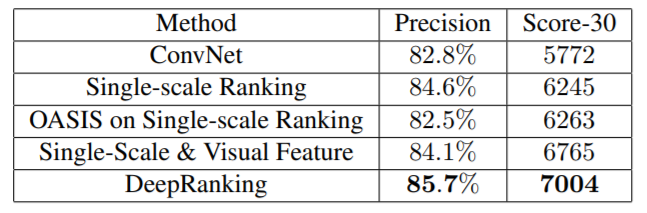
\includegraphics[scale=0.7]{img/Similarity_precision_diff_CNN}
\caption{anašumo tikslumo metrikų rezultatai \cite{Learning_fine_grained_image}} % Antraštė įterpiama po paveikslėlio
\label{img:mlp}
\end{figure}

\begin{figure}[H]
\centering
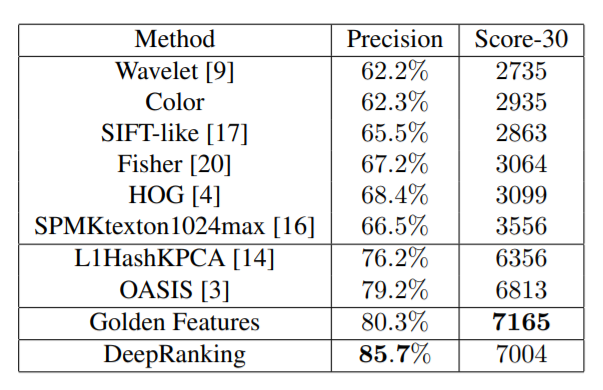
\includegraphics[scale=0.7]{img/Similarity_precision}
\caption{Panašumo tikslumo metrikų rezultatai \cite{Learning_fine_grained_image}} % Antraštė įterpiama po paveikslėlio
\label{img:mlp}
\end{figure}
\pagebreak

\section{Trejetų tinklo vaizdų atpažinimo tyrimas ir vertinimas}
\subsection{Kaip išspręsti semantines vazidų skirtumo problemas}
Norint pagerinti atsirandančias vaizdų problemas, aprašytas viršuje

\subsection{Treniravimo ir testavimo aplinka}
Trejetų tinklo modelis buvo treniruoamas naudojant Lenovo Y-700 kompiuterį su šiomis specifikacijomis: CPU i7 6700K (4 branduolių), 8GB RAM, GPU Nvidia GTX 960m (4GB RAM). Norint pasileisti trejetų modelį būtent šiam kompiuteriui (priklausomai nuo mašinos tai gali skirtis) buvo atsisiųsta Nvidia CUDA programinė įranga su tikslu, kad modelio treniravimas būtų vykdomas pasitelkiant vaizdo plokštę, o ne procesorių.
\linebreak
Priežastis kodėl buvo pasirinkta vaizdo plokštė yra todėl, kad gilusis mokymasis yra intensyvi skaičiavimo užduotis. Į gilųjį mokymasi įeina didžiuliai matricų skaičiavimai (ypač sandauga) ir kitos operacijos, kurios gali veikti paraleliai todėl vaizdo plokštė ateina į pagalbą, nes viena vaizdo plokštė gali turėti tūkstančius branduolių, tuo metu procesorius turi žymiai mažiau branduolių, nors jie ir žymiai greitesni negu vaizdo plokštės \cite{Performance_of_GPU}.
\linebreak
Pasirenktas trejetų tinklų modelis yra implementuotas naudojant Tensorflow karkasą, Python 3.5.1.
\linebreak
Vaizdų duomenų rinkinyje buvo 3884 nuotraukos, kuriose jau buvo surikiuotos teisinga eilės tvarka, kur pirma nuotrauka pagrindinė, antra nuotrauka - teigiama (kuri yra panaši į pagrindinę) bei neigiama (nepanaši į pagrindinę nuotrauką) ir tokia eilės tvarka yra išsidėstę visos kitos nuotraukos.
Ištreniravus šiuos duomenis yra bandoma analizuoti modelio tikslumą imant vaizdų pavyzdžius iš testinio duomenų rinkinio.

\subsection{VGG16 tinklo modelis}
Panaudota architektūra naudoja VGG16 tinklo bazės sluoksnius klasifikavimui todėl tik labai panašūs vaizdai gali būti naudojami duomenų treniravimui tam, kad pagerinti tinklo atlikimą bei išsaugoti skaičiavimo išteklius.
\linebreak
VGG16 yra konvoliucinių neuroninių tinklų modelis, išrastas K. Simonian ir A. Zisserman (Oksfordo universitetas). Modelis sugeba pasiekti 92.7\% top-5 testų tikslumą (treniravimo duomenys pasiimti iš ImageNet). VGG16 buvo treniruojamas savaitę iš savaitės naudojant Nvidia Titan Black vaizdo plokščių šeimas.
\subsection{Tyrimo rezultatai}
Šiame darbe buvo bandyta atpažinti detalius vaizdus, naudojant vaizdų duomenų rinkinį CUHK01. Šiame duomenų rinkinyje yra pavaizduota 3884 viešose vietose einančių pėsčiųjų kadrai. Todėl naudojant ši duomenų rinkinį buvo analizuojama, kaip su pasirinktu trejetų modeliu seksis atpažinti skirtingus žmogaus kadrus, kurie buvo nufotografuoti įvairiai -  iš kelių pusių, iš nugaros ir priekio, esant skiringai žmogaus eisenos pozicijai, skirtingam apšvietimui ir kontrastamas, įsiterpiant kitiems objektams prie pėsčiojo.
\linebreak
Ištreniravus trejetų tinklą su pasirinktu duomenų rinkiniu ir pradėjus testuoti jo rezultatus, gavau 85,7\% tikslumo rezultatą. Tai yra gan aukštas įvertinimas, nes atpažinti to paties pėsčiojo skirtingus kadras nėra lengviausia užduotis, nes susiduriame su kliūtimis, aprašytomis anksčiau.

\begin{figure}[H]
\centering
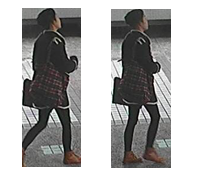
\includegraphics[scale=1.0]{img/Frame_diff.png}
\caption{Žmogaus skiringi eisenos kadrai} % Antraštė įterpiama po paveikslėlio
\label{img:mlp}
\end{figure}
\subsection{Vaizdai su prastais rezultatų palyginimais}
Visgi ne visi vaizdai buvo tesingai palyginimi ir nustatomi trejetų tinklo modelio. Todėl šiame darbe buvo ieškoma ir nagrinėjama, kurios vaizdų įvestis turėdavo prastus rezultatus bei buvo bandoma išsiaiškinti kas sukeldavo prastus rezultatus.

\begin{figure}[H]
\centering
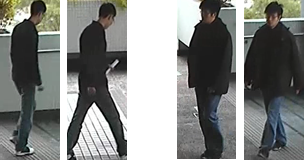
\includegraphics[scale=1.0]{img/Wrongly_detected.png}
\caption{Blogai identifikuotos vaizdų poros} % Antraštė įterpiama po paveikslėlio
\label{img:mlp}
\end{figure}

Dauguma nuotraukų, kurios buvo blogai identifikuotos skirėsi viena nuo kitos spalvų intensivimu, skirtingomis spalvomis. Pavyzdžiui matome, kad tiek pirmoje ir antroje nuotraukų porose įsiterpusi nauja žalia spalva (žalumos objektai) leidžia manyti, kad tai yra viena iš priežasčių, kodėl nepavyko tinkamai identifikuoti joms. Taip pat antroje poroje matome, kad žmogaus judėjimo kampas į objektyvą skiriasi, o ir nuotraukų šviesos intensyvumas yra kitoks. Todėl tai leidžia daryti prielaida, kad vaizdų palyginimo rezultatai bus prasti, jei nuotraukos bus nufotografuotos ne kokybiškai - apšvietimo skirtumai, netvarkingas fonas ar atsiradusi okliuzija.

\begin{figure}[H]
\centering
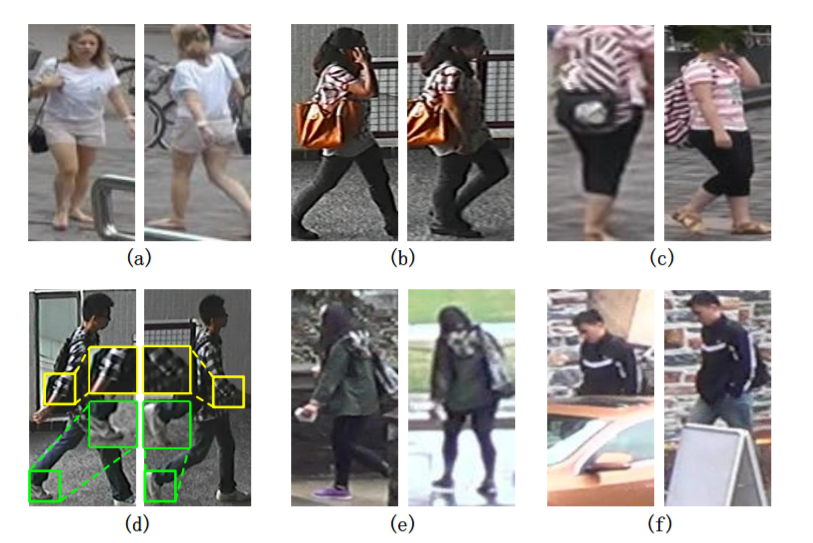
\includegraphics[scale=1.0]{img/image_diff_examples.png}
\caption{Sunkiai identifikuojamų nuotraukų poros} % Antraštė įterpiama po paveikslėlio
\label{img:mlp}
\end{figure}
Viršuje esančios žmonių nuotraukų poros yra sudėtingai identifikuojamos dėl įvairių priežasčių: a) dėl skirtngo objektyvo kampo, b) skirtingos žmogaus pozos, c) prastos nuotraukos kadro užfiksavimo (susiliejas vaizdas), d) ne vienodame lygyje esančios žmogaus kūno dalis, atsiradusios dėl jo judėjimo, e) netvarkingas fonas, f) okliuzija.

\pagebreak
\subsection{Sprendimo būdai}
Visgi ieškant literatūroje informacijos, kurioje būtų aprašyti sprendimo būdai, kai lyginami vaizdai vienas su kitu yra nekorektiški bruožų atžvilgiu, tačiau panašūs ar priklauso tai pačiai klasei, yra siūlomi keli sprendimų būdai. Pavyzdžiui, ypatybių fokusavimą nukreipiant į lokalias detales buvo sukurta nesudėtingas suskirstymas asmens nuotraukos į kelias fiksuotas ir nekintančias dalis, pavyzdžiui į horizontales juosteles ir taip mokantis lokalių nuotraukų bruožų atpažinimo. Visgi, kaip tyrimai iš literatūros nurodė toks skirstymas prastai lygina identifikuojamo asmens kūno dalis. Kituose tyrimuose ir bandymuose buvo bandoma naudoti žmogaus pozą, tokiu būdu identifikuojant skirtingas kūno dalis: kojas, rankas, veidą. Tačiau visgi ir toks atpažinimo metodas yra prastas, kad gauti norimus rezultatus, nes identifiuoti tas pačias žmogaus kūno dalis iš skirtingų žmogaus padėčių kelia problemų dėl jo skirtingos pozos nuotraukose.
\pagebreak
\section{Rezultatai ir išvados}
\thispagestyle{empty} 
\subsection{Rezultatai}
\begin{enumerate}
\item{Trejetų tinklai palyginti su Siamese modeliu, išskirti trūkumai ir privalumai.}
\item{Išskirti esamų tyrimų trūkumai}
\item{Išskirti esamų tyrimų trūkumai.}
\item{Aprašyti trjetų tinklų pasirinktas architektūros modelis.}
\end{enumerate}
\subsection{Išvados}
\begin{enumerate}
\item{Yra sudėtinga lyginti trejetų tinklų ir Siamese modelius, nes jų architektūra gali varijuota pagal tai kaip modelis yra įgyvendintas. Teisingiau yra lyginti specialius jų sukurtus modelius vienas su kitu.}
\item{Pasirinktas trejetų tinklų modelis parodė neblogus rezultatus identifikuojant žmonių eisenos kadrus.}
\item{Identifikuojant žmones nuotraukose susiduriama su rimtomis problemomis, kai to paties žmogaus nuotraukos skiriasi dėl pašalinių priežasčių. Kas lemia kad žmonių identifikacija yra sudėtingas procesas, kuris tam tikroms nuotraukoms neturi sprendimo būdų.}
\end{enumerate}
\subsection{Rekomendacijos ateities darbams}
\begin{enumerate}
\item{Išbandyti kitą trejetų modelį su pasiūlytais būdais, kurie gebėtų dar geriau atpažinti žmonių siluetus}
\item{Atlikti atpažinimo rezultatų analizę su kitis neuronų tinklais.}
\item{Ištestuoti su daugiau duomenų rinkinių. Stebėti ir lyginti rezultatus}
\item{Iškelti savo palyginimo metodą, kuris gebėtų teisingai identifikuoti žmones nuotraukose.}
\end{enumerate}
\pagebreak

\section{Priedai}
\thispagestyle{empty} 
\subsection{Žodynas}
\begin{itemize}
\item{Svoris(angl. weight) - parametras neuroniname tinkle, kuris transformuoja įvesties duomenys paslėptuose sluoksniuose.}
\item{Nuostolių funkcija(angl. loss function) - funkcija, padedanti optimizuoti svorius, taip sumažinant neatitikimų nuostolius.}
\item{Detalieji vaizdai(angl. fine-grained) - detalūs vaizdai. Vaizdo klasifikavimo užduotyse, tai yra įvesties vaizdai, kuriuos yra sudėtinga išskirti klasėms, pvz.: identifikuojant skirtingų markių automobilius.}
\item{Aktyvacijos funkcija(angl. activation function) - funkcija, skirta nustatyti ar neuronas turi būti aktyvuotas, skaičiuojant svorių sumą bei pridedant postūmio parametrą.}
\item{Postūmis(angl. bias) - papildomas parametras neuroniniuose tinkluose, kuris padeda koreguoti išvesti kartu su svorių įvesties suma, skirta neuronams perduoti. Taip pat šis parametras leidžia perstūmti aktyvacijos sumą nuo kairės į dešinę.}
\end{itemize} 
\pagebreak

\printbibliography[heading=bibintoc] 
\thispagestyle{empty}

\end{document}

